% Chapter 3: System Study
\chapter{System Study}

\section{Existing System}
Conventional washing machines available in the market fall into two main categories: semi-automatic and fully automatic machines. Both categories operate on pre-programmed cycles without the ability to adapt to specific garment requirements.

\subsection{Semi-Automatic Washing Machines}
Semi-automatic machines require significant user intervention throughout the washing process. Users must manually fill water, add detergent, transfer clothes between wash and rinse tubs, and drain water after completion. These machines offer basic timer-based controls but lack any sensing capabilities. The motor operates on fixed rotation patterns regardless of fabric type, leading to potential damage to delicate garments. Detergent quantity is left entirely to user estimation, resulting in either insufficient cleaning or excessive chemical usage.

% Figure commented out because image file not available
% \begin{figure}[H]
%     \centering
%     \includegraphics[width=0.8\textwidth]{semi_auto_controls}
%     \caption{Typical Semi-Automatic Washing Machine Controls}
%     \label{fig:semi_auto}
% \end{figure}

\subsection{Conventional Fully Automatic Machines}
Fully automatic machines eliminate manual intervention for fill, wash, and drain operations. However, they operate on fixed program cycles (Cotton, Synthetic, Delicate, Wool) that users select based on general fabric categories. These programs use predetermined parameters:
\begin{itemize}
    \item Fixed water levels regardless of load size or soil level
    \item Standardized detergent quantities (user must add manually)
    \item Pre-set wash and spin durations
    \item Uniform mechanical action within each program
\end{itemize}

Research indicates that conventional machines use 30–40\% more water than necessary for lightly soiled garments (Kumar et al., 2021). Additionally, the generalized cycles cannot account for varying soil levels, mixed fabric loads, or specific care requirements of modern textile blends.

% Figure commented out because image file not available
% \begin{figure}[H]
%     \centering
%     \includegraphics[width=0.8\textwidth]{full_auto_controls}
%     \caption{Conventional Fully Automatic Machine Program Selection}
%     \label{fig:full_auto}
% \end{figure}

\subsection{Smart Washing Machines (Commercial)}
Recent commercial offerings from LG (ThinQ with AI DD), Samsung (QuickDrive), and Whirlpool incorporate basic intelligence:
\begin{itemize}
    \item \textbf{LG AI DD:} Uses weight and fabric softness sensors to optimize wash motions. Claims to detect fabric characteristics but does not perform visual analysis.
    \item \textbf{Samsung QuickDrive:} Employs sensors to detect load size and soil level through turbidity sensing after wash begins.
    \item \textbf{Whirlpool 6th Sense:} Adjusts cycle duration based on load size and temperature.
\end{itemize}
However, these systems share common limitations:
\begin{itemize}
    \item \textbf{Proprietary Technology:} Algorithms are closed-source and non-modifiable
    \item \textbf{High Cost:} Premium pricing (INR 30,000–INR 80,000) makes them inaccessible to many households
    \item \textbf{No Visual Analysis:} Lack camera-based fabric identification capabilities
    \item \textbf{No Retrofit Option:} Require complete machine replacement
    \item \textbf{Limited Adaptability:} Cannot be customized for specific user requirements
\end{itemize}

% Figure commented out because image file not available
% \begin{figure}[H]
%     \centering
%     \includegraphics[width=0.8\textwidth]{smart_apps}
%     \caption{Commercial Smart Washing Machine Applications}
%     \label{fig:smart_apps}
% \end{figure}

\subsection{Research Prototypes}
Academic research has explored various smart laundry concepts:
\begin{itemize}
    \item Sensor-based systems using weight, turbidity, and conductivity sensors (Patil \& Deshmukh, 2022)
    \item RFID-tagged garments with pre-programmed care instructions (Chen et al., 2020)
    \item Computer vision systems for fabric classification using CNNs (Liu et al., 2021)
\end{itemize}
However, these remain laboratory prototypes without integration into functional washing machines or consideration for retrofit applications.

\subsection{Limitations of Existing Systems}
Conventional washing machines face several critical limitations across multiple aspects. In terms of fabric identification, no existing consumer machine performs true visual analysis of the garments. Parameter adaptation is also restricted, as fixed cycles cannot adjust to actual soil levels or fabric sensitivity. Furthermore, resource optimization is hindered by water and detergent usage being based on broad averages rather than specific requirements. From a financial perspective, ready-made smart machines are prohibitively expensive for many households. Additionally, there are currently no viable retrofit solutions for upgrading existing machines, and the proprietary nature of commercial systems prevents users from modifying or enhancing their appliances.

\section{Proposed System}
The proposed AI‑Integrated Washing Machine addresses the limitations of existing systems through a comprehensive retrofit solution that combines computer vision, AI‑based decision making, and automated hardware control. The system is designed to convert a conventional semi‑automatic washing machine into a fully intelligent appliance by integrating three core layers: a visual analysis layer that uses the Gemini API to identify fabric type, fiber category, and soil level from captured garment images; a reasoning layer implemented as dual FastAPI services that translate the visual data into precise washing parameters (detergent volume, water level, soak and spin times, temperature, and mechanical action); and an execution layer driven by an Arduino WiFi R4 microcontroller that autonomously controls the motor, water inlet, detergent pump, and outlet valve. A cross‑platform mobile application built with React Native provides the user interface for scanning, cycle monitoring, and manual override, completing an end‑to‑end solution that eliminates guesswork, optimizes resource usage, and extends fabric life. The architecture is modular, allowing each component to be developed, tested, and upgraded independently, while the use of a feedback loop enables continuous improvement of AI accuracy through user corrections. This approach not only delivers smart functionality at a fraction of the cost of new AI‑enabled machines but also offers a replicable blueprint for retrofitting legacy appliances.
\subsection{System Overview}
The system transforms a conventional semi-automatic washing machine into an intelligent appliance capable of:
\begin{itemize}
    \item \textbf{Visual Garment Analysis:} Scanning fabric using an integrated camera and identifying material type, fiber category, and soil level through Gemini API
    \item \textbf{Intelligent Parameter Calculation:} Determining optimal washing parameters based on fabric characteristics and soil level
    \item \textbf{Automated Hardware Control:} Executing the calculated cycle through Arduino-controlled relays, pumps, and valves
    \item \textbf{User Interface:} Providing mobile application for scanning, monitoring, and manual override
\end{itemize}

% Figure for system architecture
\begin{figure}[H]
    \centering
    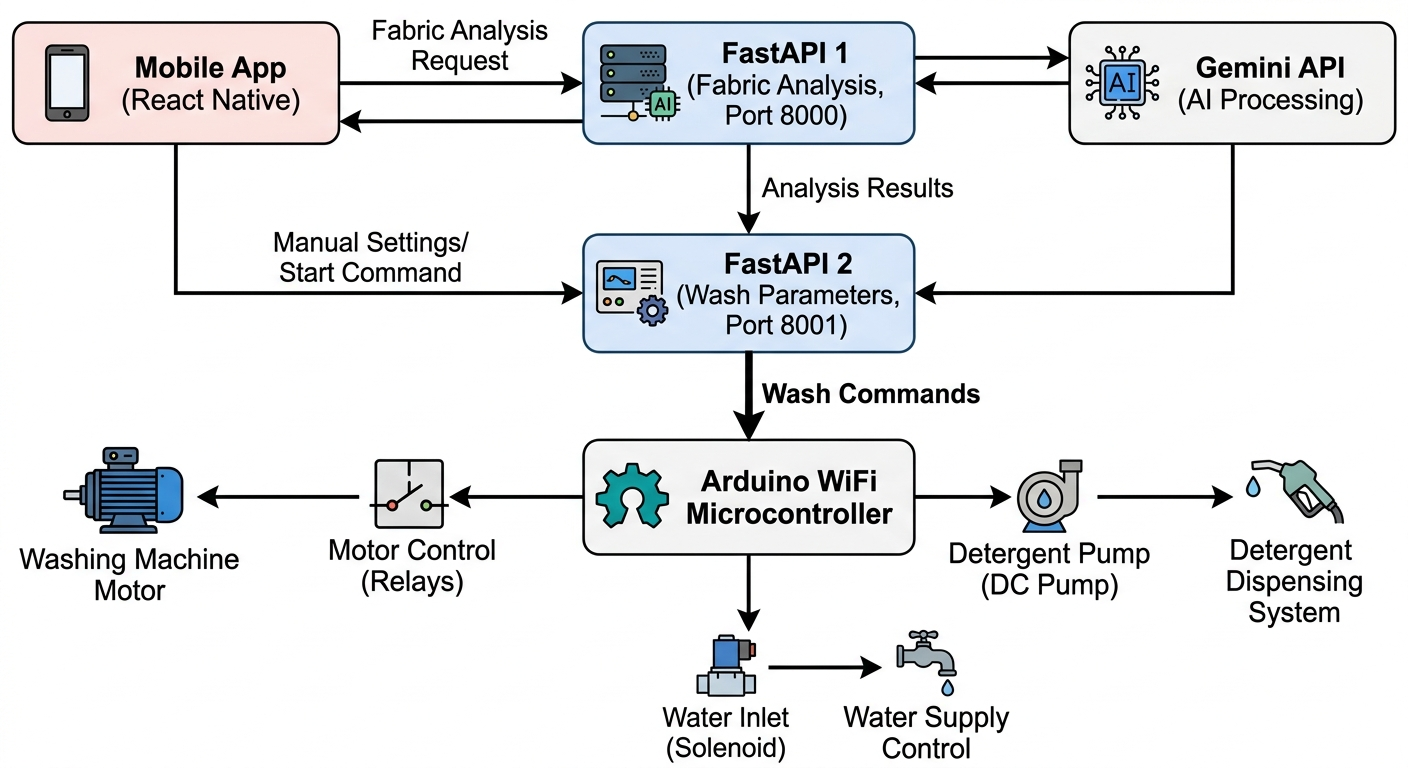
\includegraphics[width=\textwidth]{img/c3diagram1} % Architecture diagram
    \caption{Proposed System Architecture Block Diagram}
    \label{fig:architecture}
\end{figure}

\subsection{Key Components}
\textbf{Hardware Components:}
\begin{itemize}
    \item Arduino WiFi R4 (Microcontroller)
    \item 2 Relays for motor rotation control
    \item 1 Relay for solenoid water inlet valve
    \item Solenoid Water Inlet Valve
    \item 240V, 10A Three-Phase Motor (existing washing machine motor)
    \item 5V DC Water Pump (detergent dispenser)
    \item TAS122 Transistor (pump control)
    \item 12V L298N DC Motor Driver (outlet valve control)
\end{itemize}

\textbf{Software Components:}
\begin{itemize}
    \item React Native Expo Mobile Application
    \item FastAPI 1: Fabric Analysis Service (Port 8000)
    \item FastAPI 2: Wash Parameter Service (Port 8001)
    \item Arduino Firmware (C++)
\end{itemize}

\textbf{AI Components:}
\begin{itemize}
    \item Gemini API for fabric analysis
    \item Pillow Library for image processing
    \item Two-stage prompt engineering system
\end{itemize}

% Photo of complete hardware setup
\begin{figure}[H]
    \centering
    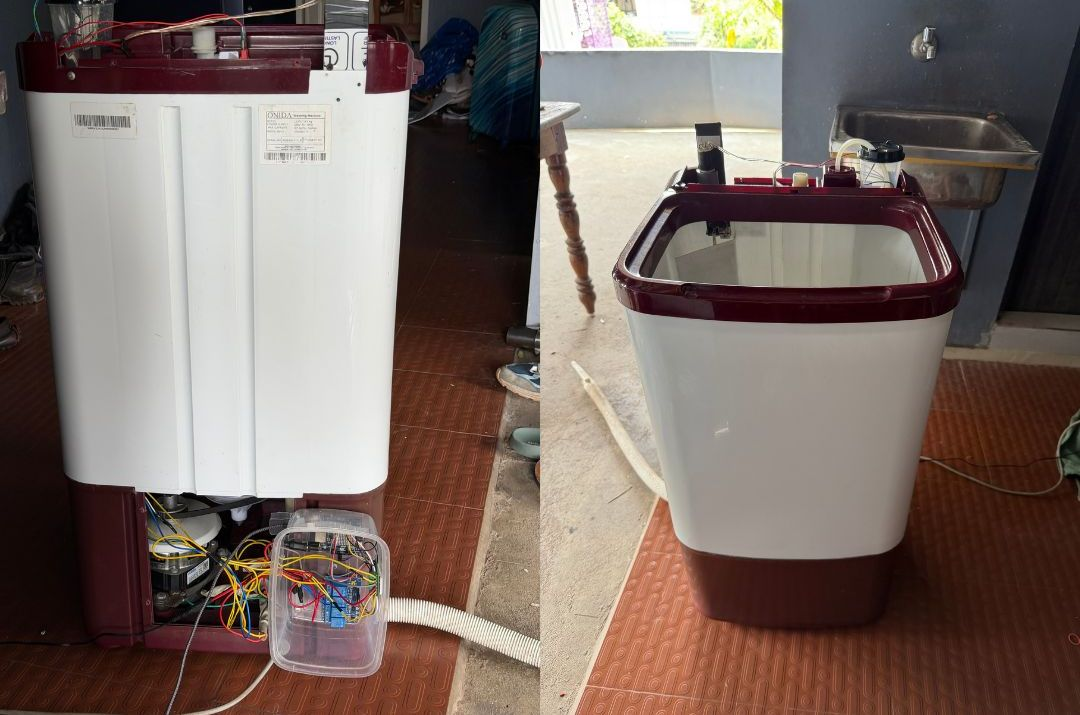
\includegraphics[width=0.8\textwidth]{img/c3diagram2} % Hardware photo
    \caption{Complete Project Hardware Setup}
    \label{fig:hardware}
\end{figure}

\subsection{System Workflow}
\begin{enumerate}
    \item User places garment on washing machine and opens mobile application
    \item Camera captures image of the fabric
    \item Image sent to FastAPI 1 which processes it using Pillow and forwards to Gemini API with Prompt 1
    \item Gemini returns fabric analysis including:
        \begin{itemize}
            \item Material type (e.g., “Cotton Twill”)
            \item Fiber category (Natural/Synthetic/Semi-synthetic)
            \item Property description
            \item Soil level (1–5)
            \item Confidence score
        \end{itemize}
    \item Output sent to FastAPI 2 which applies Prompt 2 logic to calculate washing parameters:
        \begin{itemize}
            \item Detergent amount (ml)
            \item Soak time (minutes)
            \item Spin time (minutes)
            \item Water level (liters)
            \item Wash cycles
            \item Temperature (°C)
            \item Mechanical action
        \end{itemize}
    \item Parameters transmitted to Arduino via WiFi
    \item Arduino executes cycle:
        \begin{itemize}
            \item Opens water inlet solenoid for calculated duration
            \item Activates detergent pump using linear regression timing
            \item Runs motor in programmed rotation pattern
            \item Opens outlet valve for drainage
            \item Reports status back to mobile app
        \end{itemize}
    \item User monitors progress through mobile application
\end{enumerate}

\subsection{Advantages Over Existing Systems}
The proposed AI-Integrated Washing Machine offers significant advantages over conventional systems. By utilizing the Gemini API for visual analysis, it achieves accurate and automated material detection. The system enables dynamic parameter adaptation, calculating wash settings based on the actual fabric type and soil level detected. This leads to superior resource optimization, where precise water and detergent quantities are used to minimize waste. The retrofit approach provides these smart features at a fraction of the cost of purchasing a new AI-enabled machine and is compatible with existing semi-automatic models. Its open architecture and documented APIs allow for easy customization and future enhancements, while an integrated feedback loop allows the system to improve its classification accuracy over time based on user input.

\section{Software Requirements Specification}

\subsection{Overall Description}
\subsubsection*{Product Perspective}
The AI-Integrated Washing Machine software system is a new, self-contained solution designed to retrofit existing semi-automatic washing machines. The system interfaces with:
\begin{itemize}
    \item \textbf{Hardware:} Arduino microcontroller, camera module, relays, pumps, valves
    \item \textbf{External Services:} Gemini API for AI processing
    \item \textbf{Users:} Home users operating the mobile application
    \item \textbf{Network:} WiFi for communication between components
\end{itemize}

\subsubsection*{User Characteristics}
\begin{itemize}
    \item \textbf{Primary Users:} Homeowners with basic smartphone proficiency
    \item \textbf{Technical Users:} Developers/researchers who may modify or extend the system
    \item No specialized training required for basic operation
\end{itemize}

\subsubsection*{Operating Environment}
\begin{itemize}
    \item Mobile application runs on iOS/Android devices
    \item FastAPI services run on local server or cloud host
    \item Arduino operates in household environment (temperature, humidity, vibration)
    \item WiFi network connectivity required for AI processing
\end{itemize}

\subsubsection*{Design and Implementation Constraints}
\begin{itemize}
    \item Internet connectivity required for Gemini API access
    \item Camera must have minimum resolution for fabric detail capture
    \item Arduino must handle real-time control with minimal latency
    \item Linear regression calculations must execute within microcontroller constraints
    \item Safety mechanisms must prevent hardware damage
\end{itemize}

\subsubsection*{Assumptions and Dependencies}
\begin{itemize}
    \item User has stable WiFi internet connection
    \item Gemini API remains available with consistent performance
    \item Washing machine mechanical systems are functional
    \item Power supply meets Arduino and component requirements
    \item User follows basic safety precautions for electrical appliances
\end{itemize}

\subsection{Product Functions}
The software system performs the following primary functions:

\textbf{Mobile Application Functions:}
\begin{itemize}
    \item User registration and authentication
    \item Camera interface for garment scanning
    \item Display of fabric analysis results
    \item Wash cycle parameter preview and confirmation
    \item Real-time wash progress monitoring
    \item Manual override controls for emergency situations
    \item System configuration and calibration settings
    \item Historical cycle records and fabric analysis logs
\end{itemize}

\textbf{FastAPI 1 Functions (Fabric Analysis):}
\begin{itemize}
    \item Accept image upload from mobile application
    \item Process image format using Pillow library
    \item Construct Prompt 1 with image data
    \item Invoke Gemini API for fabric analysis
    \item Parse and validate JSON response
    \item Return structured fabric data to mobile app
    \item Forward relevant data to FastAPI 2
    \item Log analysis attempts for feedback loop
\end{itemize}

\textbf{FastAPI 2 Functions (Wash Parameters):}
\begin{itemize}
    \item Accept fabric data from API 1
    \item Apply Prompt 2 logic for parameter calculation
    \item Return structured washing parameters
    \item Format parameters for Arduino transmission
    \item Validate parameter ranges for safety
\end{itemize}

\textbf{Arduino Firmware Functions:}
\begin{itemize}
    \item Receive washing parameters via WiFi
    \item Calculate detergent pump activation time using linear regression
    \item Control motor relays with programmed rotation timing
    \item Activate water inlet solenoid for calculated duration
    \item Monitor cycle progress and report status
    \item Activate outlet valve for drainage
    \item Implement safety timeouts and error detection
    \item Return real-time status to mobile application
\end{itemize}

\subsection{Software Requirements Specification}

\subsubsection{External Interfaces}
\textbf{User Interfaces:}
The mobile application provides the primary user interface with the following screens:
The mobile application is designed with several key screens to provide a comprehensive user experience. The Dashboard serves as the central hub, offering a system overview, status indicators, recent cycle history, and a quick-scan button. The Fabric Analysis screen facilitates the core functionality of garment scanning, featuring a camera viewfinder, capture controls, and a results display with confidence indicators. For active cycles, the Wash Progress screen provides real-time monitoring through progress bars, time-remaining estimates, and stage indicators. Safety and control are handled by the Manual Override screen, which includes emergency controls for stopping the motor or water flow and immediate drainage. Finally, the Settings screen allows for system configuration, including WiFi setup, calibration values, and personalized user preferences.

\textbf{Hardware Interfaces:}
\begin{table}[H]
    \centering
    \begin{tabular}{|l|l|l|}
        \hline
        \textbf{Hardware Component} & \textbf{Interface Type} & \textbf{Control Method} \\
        \hline
        Motor (CW) & Digital Output & Relay 1 (HIGH = ON) \\
        \hline
        Motor (CCW) & Digital Output & Relay 2 (HIGH = ON) \\
        \hline
        Water Inlet Solenoid & Digital Output & Relay 3 (HIGH = ON) \\
        \hline
        Detergent Pump & Digital Output & TAS122 Transistor (HIGH = ON) \\
        \hline
        Outlet Valve & PWM/Speed Control & L298N Motor Driver \\
        \hline
        Camera & USB/Wireless & Mobile device camera API \\
        \hline
    \end{tabular}
    \caption{Hardware Interfaces}
    \label{tab:hardware_if}
\end{table}

\textbf{Software Interfaces:}
% Using tabularx to avoid overfull boxes
\begin{table}[H]
    \centering
    \begin{tabularx}{\textwidth}{|l|l|l|X|}
        \hline
        \textbf{Interface} & \textbf{Protocol} & \textbf{Data Format} & \textbf{Purpose} \\
        \hline
        Mobile App -- FastAPI 1 & HTTP/REST & JSON, Multipart/Form-Data & Image upload, results \\
        \hline
        FastAPI 1 -- Gemini API & HTTPS & JSON with image encoding & AI analysis \\
        \hline
        FastAPI 1 -- FastAPI 2 & HTTP/REST & JSON & Fabric data transfer \\
        \hline
        FastAPI 2 -- Arduino & HTTP/WiFi & JSON & Wash parameters \\
        \hline
        Arduino $\rightarrow$ Mobile App & WebSocket/HTTP & JSON & Status updates \\
        \hline
    \end{tabularx}
    \caption{Software Interfaces}
    \label{tab:software_if}
\end{table}

\textbf{Communication Interfaces:}
\begin{itemize}
    \item WiFi 802.11 b/g/n for all network communication
    \item HTTP/HTTPS for REST API calls
    \item WebSocket for real-time status updates (optional)
    \item Serial (USB) for Arduino debugging and calibration
\end{itemize}

\subsubsection{Functional Requirements}
\begin{description}
    \item[FR1: User Authentication] \hfill \\
        \begin{itemize}
            \item FR1.1: System shall allow user registration with email and password
            \item FR1.2: System shall authenticate users before granting access
            \item FR1.3: System shall maintain user sessions securely
        \end{itemize}
    \item[FR2: Garment Scanning] \hfill \\
        \begin{itemize}
            \item FR2.1: System shall activate device camera for image capture
            \item FR2.2: System shall allow user to capture garment image
            \item FR2.3: System shall transmit image to FastAPI 1 for processing
        \end{itemize}
    \item[FR3: Fabric Analysis (API 1)] \hfill \\
        \begin{itemize}
            \item FR3.1: System shall accept image uploads in JPEG/PNG format
            \item FR3.2: System shall process image using Pillow library
            \item FR3.3: System shall construct Prompt 1 with appropriate context
            \item FR3.4: System shall invoke Gemini API with constructed prompt
            \item FR3.5: System shall parse Gemini response into structured JSON
            \item FR3.6: System shall return fabric analysis to mobile app
            \item FR3.7: System shall log analysis for feedback loop
        \end{itemize}
    \item[FR4: Parameter Calculation (API 2)] \hfill \\
        \begin{itemize}
            \item FR4.1: System shall accept fabric data from API 1
            \item FR4.2: System shall apply Prompt 2 logic to calculate washing parameters
            \item FR4.3: System shall validate parameters against safety limits
            \item FR4.4: System shall return parameters in specified JSON format
            \item FR4.5: System shall format parameters for Arduino transmission
        \end{itemize}
    \item[FR5: Arduino Control] \hfill \\
        \begin{itemize}
            \item FR5.1: System shall receive wash parameters via WiFi
            \item FR5.2: System shall calculate detergent pump time using linear regression: \( \text{Time} = (\text{Volume} - b) / a \)
            \item FR5.3: System shall control motor relays with pattern: 5s CW → 2s pause → 5s CCW (loop)
            \item FR5.4: System shall activate water inlet solenoid for calculated duration
            \item FR5.5: System shall activate detergent pump for calculated duration
            \item FR5.6: System shall control outlet valve for drainage
            \item FR5.7: System shall report cycle status to mobile app
        \end{itemize}
    \item[FR6: Manual Override] \hfill \\
        \begin{itemize}
            \item FR6.1: System shall provide emergency stop for all operations
            \item FR6.2: System shall allow manual drain activation
            \item FR6.3: System shall allow manual pump control for calibration
        \end{itemize}
    \item[FR7: Feedback and Logging] \hfill \\
        \begin{itemize}
            \item FR7.1: System shall record all fabric analyses with confidence scores
            \item FR7.2: System shall allow user correction of misclassifications
            \item FR7.3: System shall use corrected data for prompt refinement
        \end{itemize}
\end{description}

\subsubsection{Non-Functional Requirements}

\begin{center}
\begin{longtable}{|p{3.5cm}|p{10cm}|}
\caption{Non-Functional Requirements}
\label{tab:nfr}\\
\hline
\textbf{Requirement} & \textbf{Target} \\
\hline
\endfirsthead

\multicolumn{2}{c}%
{{\bfseries \tablename\ \thetable{} -- continued from previous page}} \\
\hline
\textbf{Requirement} & \textbf{Target} \\
\hline
\endhead

\hline \multicolumn{2}{r}{{Continued on next page}} \\ \hline
\endfoot

\hline
\endlastfoot

% NFR1: Performance
\multicolumn{2}{|c|}{\textbf{NFR1: Performance}} \\
\hline
Image capture to analysis results & $<$ 5 seconds \\
\hline
API response time (internal) & $<$ 500 ms \\
\hline
Gemini API response time & $<$ 3 seconds \\
\hline
Arduino command execution & $<$ 100 ms \\
\hline
Concurrent users supported & Minimum 10 \\
\hline

% NFR2: Reliability
\multicolumn{2}{|c|}{\textbf{NFR2: Reliability}} \\
\hline
System uptime & 99\% (excluding network/API dependencies) \\
\hline
Mean time between failures & $>$ 100 cycles \\
\hline
Graceful degradation & Manual mode available if AI services unavailable \\
\hline
Data persistence & No loss of user settings or calibration data \\
\hline

% NFR3: Availability
\multicolumn{2}{|c|}{\textbf{NFR3: Availability}} \\
\hline
Core washing functions & Available even without internet (manual mode) \\
\hline
API services & Targeted for 24/7 availability \\
\hline
Automatic reconnection & On network interruption \\
\hline

% NFR4: Security
\multicolumn{2}{|c|}{\textbf{NFR4: Security}} \\
\hline
API keys & Stored as environment variables, never in code \\
\hline
WiFi communication & Secured with WPA2 \\
\hline
User data & No sensitive data stored permanently \\
\hline
Input validation & On all API endpoints \\
\hline
Rate limiting & To prevent abuse \\
\hline

% NFR5: Safety
\multicolumn{2}{|c|}{\textbf{NFR5: Safety}} \\
\hline
Motor control relays & Normally open (fail-safe) \\
\hline
Maximum continuous motor operation & 30 minutes (thermal protection) \\
\hline
Water inlet & Fails closed on power loss \\
\hline
Detergent pump & Fails off on power loss \\
\hline
Software watchdogs & Monitor Arduino responsiveness \\
\hline
Emergency stop & Overrides all operations \\
\hline

% NFR6: Usability
\multicolumn{2}{|c|}{\textbf{NFR6: Usability}} \\
\hline
Mobile app & No training required for basic operation \\
\hline
Controls & Clearly labeled with intuitive icons \\
\hline
Confirmation dialogs & For destructive actions \\
\hline
Progress indicators & For all operations \\
\hline
Error messages & In plain language with recovery suggestions \\
\hline

% NFR7: Maintainability
\multicolumn{2}{|c|}{\textbf{NFR7: Maintainability}} \\
\hline
Code documentation & Comments and README files \\
\hline
Modular architecture & Allows component replacement \\
\hline
Configuration & Stored separately from code \\
\hline
Version control & Git for all software components \\
\hline
API documentation & OpenAPI/Swagger \\
\hline

% NFR8: Scalability
\multicolumn{2}{|c|}{\textbf{NFR8: Scalability}} \\
\hline
API services & Designed for horizontal scaling \\
\hline
Architecture & Stateless enables load balancing \\
\hline
Database design & Accommodates multiple users \\
\hline
Arduino firmware & Supports updates over WiFi \\
\hline

% NFR9: Accuracy
\multicolumn{2}{|c|}{\textbf{NFR9: Accuracy}} \\
\hline
Fabric classification confidence & $>$85\% \\
\hline
Detergent dispensing accuracy & $\pm$2 ml \\
\hline
Water level accuracy & $\pm$0.5 liters \\
\hline
Timing accuracy & $\pm$1 second \\
\hline

% NFR10: Regulatory Compliance
\multicolumn{2}{|c|}{\textbf{NFR10: Regulatory Compliance}} \\
\hline
Electrical safety & Compliance with local standards \\
\hline
CE/FCC certification & Considerations for commercial deployment \\
\hline
Data privacy & GDPR compliance for European users \\
\hline

\end{longtable}
\end{center}

% NO \end{document} HERE – this file is meant to be \include'd